\section{图像分类classification.cpp}
该例子程序实现了通过Caffe进行图像分类的功能,在使用中需要借助OpenCV的帮助以实现图像的读写操作。下面来学习具体的实现过程。
\begin{minted}{c++}
#include <caffe/caffe.hpp>
#ifdef USE_OPENCV
#include <opencv2/core/core.hpp>
#include <opencv2/highgui/highgui.hpp>
#include <opencv2/imgproc/imgproc.hpp>
#endif  // USE_OPENCV
#include <algorithm>
#include <iosfwd>
#include <memory>
#include <string>
#include <utility>
#include <vector>
\end{minted}
在Caffe中,所用的核心功能都已经编译为一个动态链接库,使用该库需要首先将Caffe的头文件caffe/caffe.hpp包含进来。接着可以看到一个包含OpenCV的与编译宏,然后是一些使用到的头文件。
\begin{minted}{c++}
#ifdenf USE_OPENCV
...
#else
int main(int argc, char** argv) {
  LOG(FATAL) << "This example requires OpenCV; compile with USE_OPENCV.";
}
#endif  // USE_OPENCV
\end{minted}
其实这个程序的整个代码都被写在一个预编译宏中,用来强调对OpenCV的依赖。
在保证可以满足OpenCV依赖之后,程序使用caffe命名空间和string域,并定义一个pair类型变量,用来存贮分类的结果和得分。
\begin{minted}{c++}
using namespace caffe;  // NOLINT(build/namespaces)
using std::string;

/* Pair (label, confidence) representing a prediction. */
typedef std::pair<string, float> Prediction;
\end{minted}

\subsection{Classifier类的声明}
Classifier类是分类功能的核心部分,也是整个程序中唯一的类,其声明部分代码如下:
\begin{minted}{c++}
class Classifier {
 public:
  Classifier(const string& model_file,
             const string& trained_file,
             const string& mean_file,
             const string& label_file);

  std::vector<Prediction> Classify(const cv::Mat& img, int N = 5);

 private:
  void SetMean(const string& mean_file);

  std::vector<float> Predict(const cv::Mat& img);

  void WrapInputLayer(std::vector<cv::Mat>* input_channels);

  void Preprocess(const cv::Mat& img,
                  std::vector<cv::Mat>* input_channels);

 private:
  shared_ptr<Net<float> > net_;
  cv::Size input_geometry_;
  int num_channels_;
  cv::Mat mean_;
  std::vector<string> labels_;
};
\end{minted}

从声明中可也看出,该类的构造函数需要输入4个参数,如表\ref{chp-examples-classification-cpp1}所示,这些文件也是Caffe学习中常用到的一些文件,他们是Caffe能够正常运行的重要部分,也是机器学习中的用来调整参数的重要文件。
\begin{cntable}{参数}{chp-examples-classification-cpp1}
  \begin{tabular}{|c|l|}
    \hline
    model\_file & 网络模型定义文件 \\ \hline
    trained\_file & 训练好的模型文件 \\ \hline
    mean\_fiel & 数据均值文件 \\ \hline
    label\_file & 保存标记的文件 \\
    \hline
  \end{tabular}
\end{cntable}

\subsection{构造函数}
Classifier类的定义已经在前文做了简要说明,下边对该类进行拆分,并对其中的成员做一一介绍。

\begin{minted}{c++}
#ifdef CPU_ONLY
  Caffe::set_mode(Caffe::CPU);
#else
  Caffe::set_mode(Caffe::GPU);
#endif
\end{minted}
在构造函数中以预编译宏的方式,通过调用Caffe内建方法set\_mode()来控制程序运行是否使用GPU。
\begin{minted}{c++}
  /* Load the network. */
  net_.reset(new Net<float>(model_file, TEST));
  net_->CopyTrainedLayersFrom(trained_file);

  CHECK_EQ(net_->num_inputs(), 1) << "Network should have exactly one input.";
  CHECK_EQ(net_->num_outputs(), 1) << "Network should have exactly one output.";

  Blob<float>* input_layer = net_->input_blobs()[0];
  num_channels_ = input_layer->channels();
  CHECK(num_channels_ == 3 || num_channels_ == 1)
    << "Input layer should have 1 or 3 channels.";
  input_geometry_ = cv::Size(input_layer->width(), input_layer->height());
\end{minted}
对Classifier类中的私有成员指针型变量shared\_ptr<Net<float> > net\_进行构造,该变量指的是Caffe中的神经网络结构(由Caffe的Net类管理),在类中使用了Boost库的Shared\_ptr智能指针。在Net类的构造中需要指定model\_file参数和运行类型为TEST模式(因为不需要进行网络训练),然后使用reset()方法将net\_指针指向一个新构造的Net对象。获得网络结构后,使用Net类的CopyTrainedLayersFrom(trained\_file)方法将训练好的模型加载(拷贝)到该网络,然后使用gtest库的CHECK\_EQ()方法对输入和输出层数进行检查,如果二者不相等,那么程序运行就会被终止并输出错误说明。


为了获得输入图像的相关信息,定义一个Blob<float>类型的指针变量input\_layer并指向网络的第一个输入blob,(通过Net类的input\_blobs()方法可以获得输入层的所有blob地址所组成的数组的指针,然后取数组中第一个地址中的值,也就是指向第一个blob的指针,这里要注意的是一个blob对象可以存储多副图像)。接着就可以通过input\_layer变量获得输入图像的通道数input\_layer->channels(),并将该值存入Classifier类的成员变量num\_channels\_中,然后检查通道数是否为3或者1。对于图像的尺度,可以使用OpenCV库的Size方法,构造一个Size对象用来存储。

\begin{minted}{c++}
/* Load the binaryproto mean file. */
  SetMean(mean_file);
\end{minted}
使用Calssifier类的Setmean()方法加载均值文件,用来将输入图像数据进行中心化。这个方法在后文会详细讲解。

\begin{minted}{c++}
/* Load labels. */
  std::ifstream labels(label_file.c_str());
  CHECK(labels) << "Unable to open labels file " << label_file;
  string line;
  while (std::getline(labels, line))
    labels_.push_back(string(line));

  Blob<float>* output_layer = net_->output_blobs()[0];
  CHECK_EQ(labels_.size(), output_layer->channels())
    << "Number of labels is different from the output layer dimension.";
\end{minted}
定义ifstream流对象labels来获取标签文件,使用gtest的CHECK检查文件是否正差打开。使用getline()函数获得标签文件中的每一行并存入预先定义的line字符串中,然后将其按行压入Classifier类的成员变量labels\_中,该变量定义为一个元素为字符串的向量std::vector<string> labels\_。


定义一个Blob型的指针变量output\_layer指向网络的输出net\_->output\_blobs()[0],然后检查label的个数是否与输出blob的通道数相同,该值事实上就是分类的类别数。

\subsection{预测结果排序}
Caffe对一副图像的类别进行预测的结果是该图像属于不同类别的概率值(也可以看作一个打分),数值越大则该图像隶属于对应类别的可能性越高。因此在预测结束后需要对每个类别的隶属分数进行一个排序,将对应分数最高的类别定为最终的分类结果。


\begin{minted}{c++}
static bool PairCompare(const std::pair<float, int>& lhs,
                        const std::pair<float, int>& rhs) {
  return lhs.first > rhs.first;
}

/* Return the indices of the top N values of vector v. */
static std::vector<int> Argmax(const std::vector<float>& v, int N) {
  std::vector<std::pair<float, int> > pairs;
  for (size_t i = 0; i < v.size(); ++i)
    pairs.push_back(std::make_pair(v[i], i));
  std::partial_sort(pairs.begin(), pairs.begin() + N, pairs.end(), PairCompare);

  std::vector<int> result;
  for (int i = 0; i < N; ++i)
    result.push_back(pairs[i].second);
  return result;
}
\end{minted}
程序中使用的排序方法间接用到了C/C++的标准库函数partial\_sort(),该函数可以按照一个预定义的方法对std::vector中的对象元素进行排序,该预定义方法的返回值是一个bool值。在本程序中,预定义的方法即为PairCompare(),该方法按照pair结构中第一个值的大小顺序对两个pair对象进行排序。方法Argmax()首先使用std::make\_pair()构造pair对象(pair中的第一个值类别对应的float型得分分数,第二个值为int型类别序号),然后使用partial\_sort()对vector中的pair对象进行排序,排序后的vector中的前N个值对应由PairCompare()方法得到的最大的N个pair,最后构造一个vector<int>型变量result用来存储排序后pair中的类别序号部分,并返回该result。在这里,方法PairCompare()和Argmax()都是静态方法,因此不属于Classifier类。

\subsection{对图像进行预测}
\begin{minted}{c++}
/* Return the top N predictions. */
std::vector<Prediction> Classifier::Classify(const cv::Mat& img, int N) {
  std::vector<float> output = Predict(img);

  N = std::min<int>(labels_.size(), N);
  std::vector<int> maxN = Argmax(output, N);
  std::vector<Prediction> predictions;
  for (int i = 0; i < N; ++i) {
    int idx = maxN[i];
    predictions.push_back(std::make_pair(labels_[idx], output[idx]));
  }

  return predictions;
}
\end{minted}
Classifier的Classify()函数将对一副由OpenCV读取的图像进行类别预测,并返回一个vector<Prediction>类型的预测结果。Classify()函数内部将调用另一个成员函数Predict()以得到图像在每个类别上的得分,然后通过Argmax()函数对得分进行排序并返回前N个最大得分所对应的序号,根据序号和得分构造一个vector<Prediction> predictions类型的变量,用来存储前N个标签名称和对应得分值。注意,Prediction类型已经在程序文件开始处进行了定义。

\subsection{均值文件的读取}
对于均值文件的读取和格式转换,在Classifier类的成员函数SetMean()中主要分为三个步骤:
\begin{minted}{c++}
BlobProto blob_proto;
  ReadProtoFromBinaryFileOrDie(mean_file.c_str(), &blob_proto);
\end{minted}
首先是定义一个BlobProto型变量blob\_proto,然后调用ReadProtoFromBinaryFileOrDie()函数读取均值文件并将数据存入blob\_proto变量中。

\begin{minted}{c++}
/* Convert from BlobProto to Blob<float> */
  Blob<float> mean_blob;
  mean_blob.FromProto(blob_proto);
  CHECK_EQ(mean_blob.channels(), num_channels_)
    << "Number of channels of mean file doesn't match input layer.";
\end{minted}
第二步是使用Blob类型的FromProto函数,将上步读取的BlobProto类型数据转换为Blob类型数据,并存入mean\_blob中。

\begin{minted}{c++}
/* The format of the mean file is planar 32-bit float BGR or grayscale. */
  std::vector<cv::Mat> channels;
  float* data = mean_blob.mutable_cpu_data();
  for (int i = 0; i < num_channels_; ++i) {
    /* Extract an individual channel. */
    cv::Mat channel(mean_blob.height(), mean_blob.width(), CV_32FC1, data);
    channels.push_back(channel);
    data += mean_blob.height() * mean_blob.width();
\end{minted}
第三步也是完成一个类型转换功能,将存入mean\_blob变量中的Blob类型数据转换为OpenCV中的Mat类型数据,这里直接使用了Mat类型的构造函数,通过传入Mat的长度、宽度和数据指针的方式对每个通道的数据进行存储转换,流程如图\ref{classification_cpp_binaryproto_to_mat}。注意这里用到了Blob类型的数据指针函数mutable\_cpu\_data(),具体细节将在后续章节介绍。
\begin{cnfigure}{binaryproto文件读取流程}{classification_cpp_binaryproto_to_mat}
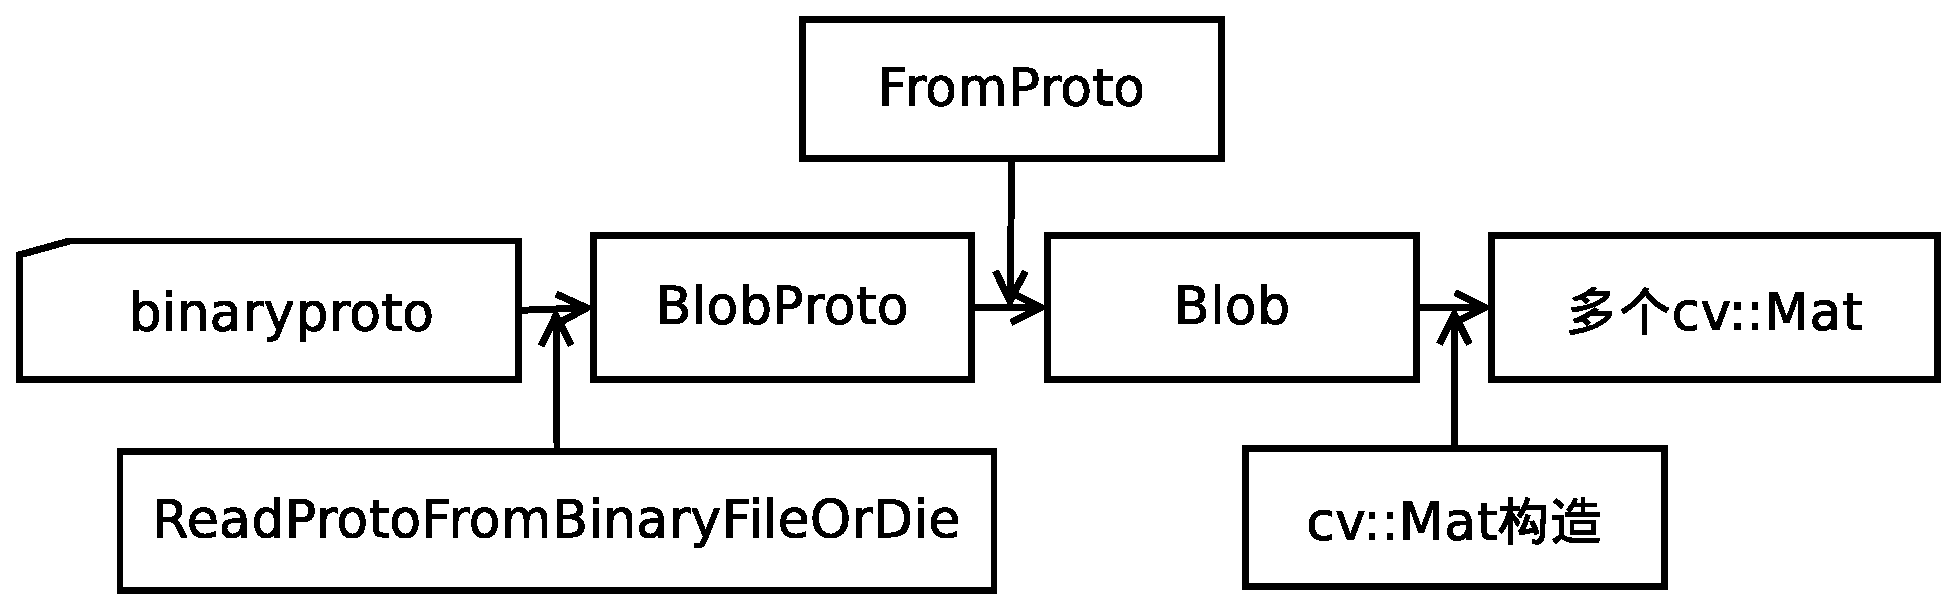
\includegraphics[height=5cm ,width=15cm,angle=0]{include/chp_from_examples/figures/classification_cpp_binaryproto_to_mat.eps}
\end{cnfigure}

完成以上三步的数据读取之后,均值数据已经分通道存储为OpenCV的Mat类型,存储变量为std::vector<cv::Mat> channels。接下来要利用OpenCV求取真正的均值并生成一个多通道Mat格式文件。
\begin{minted}{c++}
/* Merge the separate channels into a single image. */
  cv::Mat mean;
  cv::merge(channels, mean);
\end{minted}
cv::merge()方法将多个Mat融合为一个多通道Mat,存储在mean变量中。
\begin{minted}{c++}
/* Compute the global mean pixel value and create a mean image
   * filled with this value. */
  cv::Scalar channel_mean = cv::mean(mean);
  mean_ = cv::Mat(input_geometry_, mean.type(), channel_mean);
}
\end{minted}
cv::mean()方法对mean中的每个通道求取均值,返回的结果存储在cv::Scalar类型变量channel\_mean中,并使用该变量和cv::Mat的构造函数生成最终需要的均值Mat,结果存储到Classifier类的成员变量mean\_中。

\subsection{预测函数}
Classifier类的成员函数Predict()可以完成对一副图像的预测,输出每个类别的得分。
\begin{minted}{c++}
std::vector<float> Classifier::Predict(const cv::Mat& img) {
  Blob<float>* input_layer = net_->input_blobs()[0];
  input_layer->Reshape(1, num_channels_,
                       input_geometry_.height, input_geometry_.width);
  /* Forward dimension change to all layers. */
  net_->Reshape();

  std::vector<cv::Mat> input_channels;
  WrapInputLayer(&input_channels);

  Preprocess(img, &input_channels);

  net_->Forward();

  /* Copy the output layer to a std::vector */
  Blob<float>* output_layer = net_->output_blobs()[0];
  const float* begin = output_layer->cpu_data();
  const float* end = begin + output_layer->channels();
  return std::vector<float>(begin, end);
}
\end{minted}
首先获得网络输入层Blob对象的指针Blob<float>* input\_layer,通过该指针对输入层的Blob对象进行一次Reshape操作input\_layer->Reshape(1, num\_channels\_, input\_geometry\_.height, input\_geometry\_.width),注意,由于输入图像只有一副,因此第一个参数是1。然后执行net\_->Reshape对整个网络进行一次Reshape。接下来要将图像数据送入网络,这里首先使用WrapInputLayer(\&input\_channels)对网络的输入部分构造一个wrap(见后文介绍),目标是简化输入过程,然后调用Preprocess()方法,对输入图像进行预处理,以满足网络正常运行的要求,最后调用net\_->Forward()进行一次前向过程,得到网络输出。使用Blob<float>* output\_layer = net\_->output\_blobs()[0]获得输出Blob对象指针,然后根据通道数分别得到数据部分的开头和结尾处指针,最后根据两处指针的位置构造一个vector<float>(begin, end)对象并返回,其中存储的便是对应每个类别的得分值。

\subsection{对输入Blob进行包裹}
此处是整个程序代码的一个亮点,在使用Caffe时很值得借鉴。
\begin{minted}{c++}
void Classifier::WrapInputLayer(std::vector<cv::Mat>* input_channels) {
  Blob<float>* input_layer = net_->input_blobs()[0];

  int width = input_layer->width();
  int height = input_layer->height();
  float* input_data = input_layer->mutable_cpu_data();
  for (int i = 0; i < input_layer->channels(); ++i) {
    cv::Mat channel(height, width, CV_32FC1, input_data);
    input_channels->push_back(channel);
    input_data += width * height;
  }
}
\end{minted}
首先获得网络输入层的Blob对象指针,并获得该对象中的数据指针存入input\_data。对于每一个数据通道,构造cv::Mat对象(每个Mat对象的数据通过input\_data指针获得),依次将对象压入函数参数vector<cv::Mat>* input\_channels中,如图\ref{classification_cpp_wrap}这样就在网络的输入Blob和vector<cv::Mat>之间构建了一座桥梁,在使用中,只要对input\_channels指向的数据进行修改,就等价于对网络输入层的Blob对象的数据部分进行了修改。这种思路很值得借鉴。
\begin{cnfigure}{Wrap示意图}{classification_cpp_wrap}
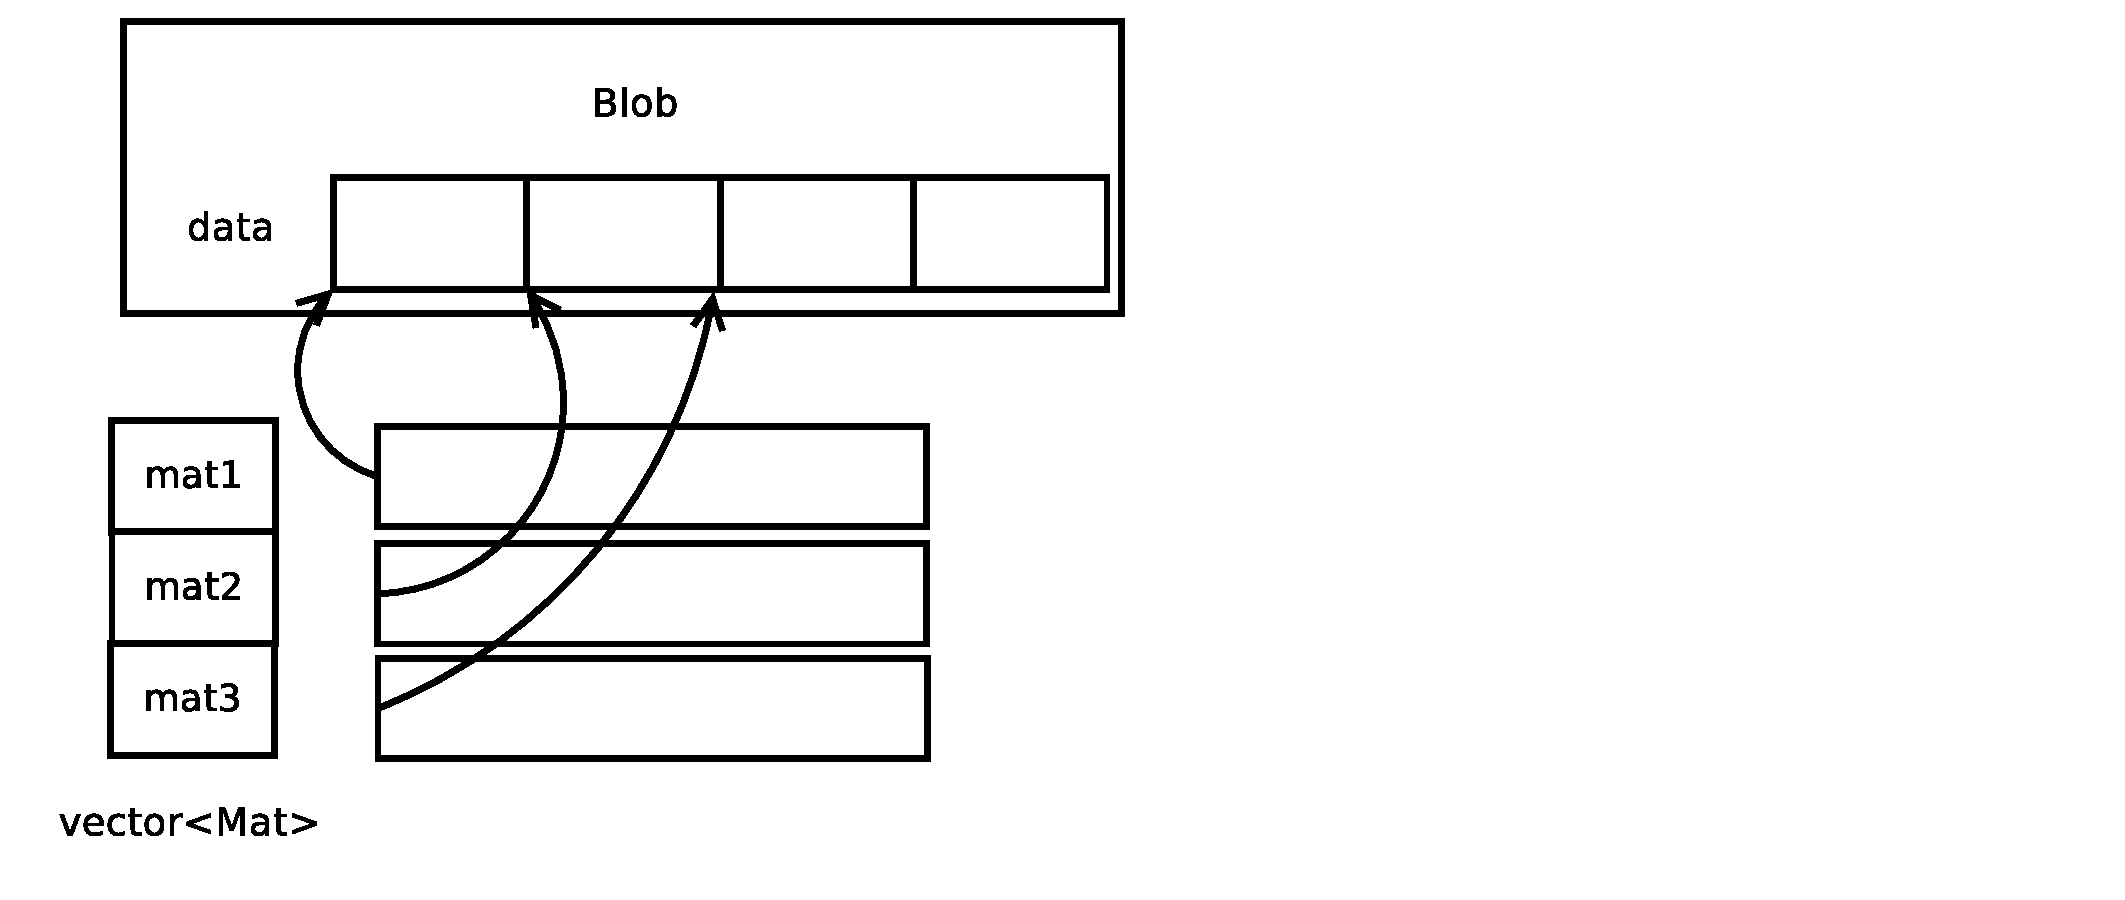
\includegraphics[height=6cm ,width=14cm,angle=0]{include/chp_from_examples/figures/classification_cpp_wrap.eps}
\end{cnfigure}


\subsection{图像预处理}
Classifier类的Preprocess()成员函数完成对输入图像的预处理,使得处理后的图像能够满足网络运行的需要。这里所有的处理操作都是通过OpenCV库来完成的。
\begin{minted}{c++}
/* Convert the input image to the input image format of the network. */
cv::Mat sample;
if (img.channels() == 3 && num_channels_ == 1)
  cv::cvtColor(img, sample, cv::COLOR_BGR2GRAY);
else if (img.channels() == 4 && num_channels_ == 1)
  cv::cvtColor(img, sample, cv::COLOR_BGRA2GRAY);
else if (img.channels() == 4 && num_channels_ == 3)
  cv::cvtColor(img, sample, cv::COLOR_BGRA2BGR);
else if (img.channels() == 1 && num_channels_ == 3)
  cv::cvtColor(img, sample, cv::COLOR_GRAY2BGR);
else
  sample = img;
\end{minted}
首先对图像的通道数进行转换,其中num\_channels\_是由读入的网络定义文件确定的,因此其目的是将图像通道数转换为与网络定义输入文件通道数一至。这里使用了cv::cvtColor()方法

\begin{minted}{c++}
cv::Mat sample_resized;
if (sample.size() != input_geometry_)
  cv::resize(sample, sample_resized, input_geometry_);
else
  sample_resized = sample;
\end{minted}
input\_geometry\_是cv::Size类型,其中存储了网络结构定义的输入图像的长度和宽度,如果真实图像与所需不符,那么就进行转换。这里使用了cv::resize()方法。

\begin{minted}{c++}
cv::Mat sample_float;
if (num_channels_ == 3)
  sample_resized.convertTo(sample_float, CV_32FC3);
else
  sample_resized.convertTo(sample_float, CV_32FC1);
\end{minted}
将图像数据从int型转换为float型。这里使用了cv::Mat类的convertTo()方法。

\begin{minted}{c++}
cv::Mat sample_normalized;
cv::subtract(sample_float, mean_, sample_normalized);
\end{minted}
对图像进行中心化,使用cv::subtract()方法,减去均值mean\_。

\begin{minted}{c++}
cv::split(sample_normalized, *input_channels);
\end{minted}
通过cv::splite()方法,将cv::Mat型数据按通道分别存储到vector<cv::Mat>* input\_channels中,由于这里经过Wrap处理,因此input\_channels已经与输入层的Blob对象绑定,该操作也就直接将图像数据传入到了网络输入层,全部流程如图\ref{classification_cpp_image_transform}。
\begin{cnfigure}{图像变换流程}{classification_cpp_image_transform}
  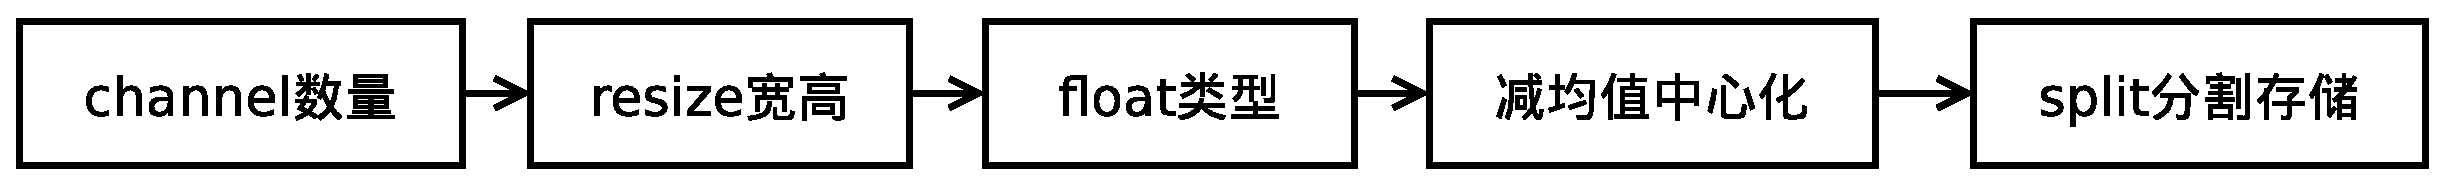
\includegraphics[height=1cm ,width=15cm,angle=0]{include/chp_from_examples/figures/classification_cpp_image_transform.eps}
\end{cnfigure}

\begin{minted}{c++}
CHECK(reinterpret_cast<float*>(input_channels->at(0).data)
        == net_->input_blobs()[0]->cpu_data())
    << "Input channels are not wrapping the input layer of the network.";
\end{minted}
在最后阶段,检查包裹过程是否成功,这里使用了C/C++标准库的reinterpret\_cast<>()方法进行类型转换,判断input\_channels中第一个Mat的数据首地址是否与网络输入层中Blob对象的数据首地址一至。


\subsection{主函数}
\begin{minted}{c++}
if (argc != 6) {
  std::cerr << "Usage: " << argv[0]
            << " deploy.prototxt network.caffemodel"
            << " mean.binaryproto labels.txt img.jpg" << std::endl;
  return 1;
}
\end{minted}
主函数中,首先检查输入参数是否为6个,这里要注意第一个参数永远为是程序本身。

\begin{minted}{c++}
::google::InitGoogleLogging(argv[0]);
\end{minted}
由于程序要用到glog库,因此在这里进行一个初始化,初始化所用到的参数为程序名本身,也就是argv[0]。

\begin{minted}{c++}
string model_file   = argv[1];
string trained_file = argv[2];
string mean_file    = argv[3];
string label_file   = argv[4];
Classifier classifier(model_file, trained_file, mean_file, label_file);
\end{minted}
处理每一个传入的参数,并使用这些参数初始化一个Classifier对象。

\begin{minted}{c++}
string file = argv[5];

std::cout << "---------- Prediction for "
          << file << " ----------" << std::endl;

cv::Mat img = cv::imread(file, -1);
CHECK(!img.empty()) << "Unable to decode image " << file;
std::vector<Prediction> predictions = classifier.Classify(img);
\end{minted}
最后一个参数(第5个参数)是要进行预测的图像文件路径。使用OpenCV的cv::imread()函数读取该图像文件,然后调用Classifier类对象的Classify()方法对图像类别进行预测,返回前N个(程序默认为前5个)得分最大的类别结果和分数。

\begin{minted}{c++}
for (size_t i = 0; i < predictions.size(); ++i) {
  Prediction p = predictions[i];
  std::cout << std::fixed << std::setprecision(4) << p.second << " - \""
            << p.first << "\"" << std::endl;
  }
\end{minted}
打印返回的结果,并在输出时设定格式和精度std::cout << std::fixed << std::setprecision(4)。
